\section{SQL Support Architectural Overview}
\label{sec:designsql}

In this section we provide an overview of a preliminary, and final architectural approaches designed in this diploma thesis, in order to support a transparent data access to backend \ac{SQL} databases. We first expose the integration approaches we should consider, and the main problems found when implementing the first approach which led us to design a second architectural approach. 


\subsection{Integration}

%integration of osgi and jbi in terms of messaging
%integration of osgi and jbi in terms of containers and libraries
%explain why we have two approaches
%jbi components offered in servicmix are deployed as osgi bundles
% jbi components offered in servicemix-mt are deployed as jbi component, and internally wrapped into an osgi bundle
% may have to put a figure of the contents in both of the packages so that we can see. It is all about the meta inf library where the bundle manifest info is exposed
As described in Chapter \ref{chap:spec}, we build the new components in ServiceMix-mt following the \ac{OSGi} compliance. However, these must interact with components which follow the \ac{JBI} specification. The integration between components built for different containers in ServiceMix-mt must be done at two levels: messaging, and resources sharing. The ServiceMix-mt \ac{NMR} \ac{API} \ac{OSGi} bundle exposes a set of operations for sending messages through the \ac{NMR} to a specified target endpoint. Hereby we can perform message exchanges between endpoints configured on \ac{OSGi} bundles and endpoints configured on \ac{JBI} components, and provide communication support between components hosted in the two containers. 

\begin{figure}[htb]
	\centering
		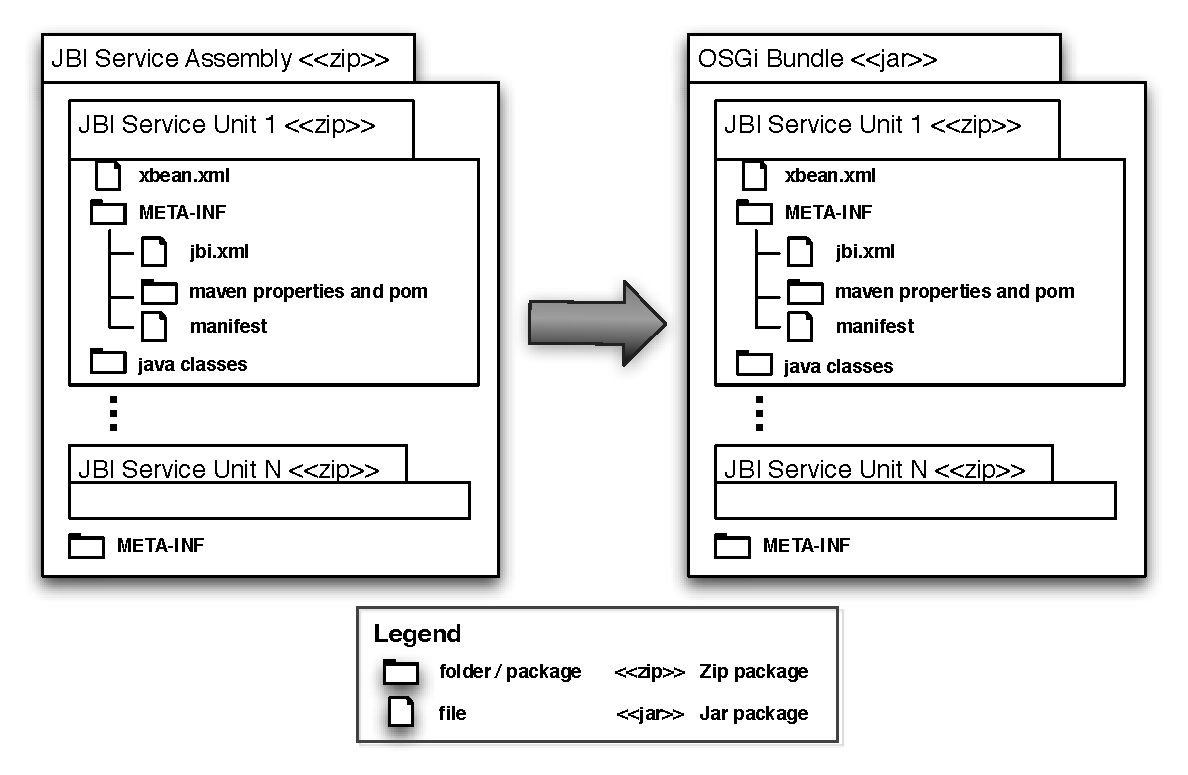
\includegraphics[clip, scale=0.5]{./gfx/osgibundlepackage.pdf}
	\caption[JBI to OSGi repackaging]{ServiceMix 4.x repackaging mechanism for deploying \ac{JBI} components in \ac{OSGi} container.}
	\label{fig:jbitoosgipackage}
\end{figure}

The resources sharing integration level refers to the deployment of \ac{JBI} components in the \ac{OSGi} container, and the utilization of packages exposed by \ac{OSGi} bundles in the \ac{OSGi} container in a loosely coupled manner. The former is part of the integration between containers provided in ServiceMix 4.x versions and described in Figure \ref{fig:jbitoosgipackage}. The deployment mechanism of a \ac{JBI} \ac{SA} into an \ac{OSGi} container is simple: repackaging of the \ac{SA} as a JAR. However, this cannot be consider a full integration in the \ac{OSGi} container. \ac{OSGi} bundles contain in their \term{META-INF} folder one fundamental file for the \ac{OSGi} kernel: the \term{manifest} file. This contains a description of the bundle, the packages it imports, and exports. Imported packages can be either statically stored in the bundle or imported from third party bundles, and exported packages are the ones which exposed to third party bundles. These can be imported with an internal class loading mechanisms developed in the \ac{OSGi} container. The repackaging of the \ac{SA} into a JAR, as it is shown in Figure \ref{fig:jbitoosgipackage}, contains the \term{META-INF} folder, and the \term{manifest} file. However, the latter only contains information about the author, date of creation, but it does not contain information related to the exported packages, and the needed packages to be imported. This \term{manifest} file describes the \ac{SA}, and not the \ac{SU}s. Java classes and package importing description are contained in the \ac{SU} package, and not in the \ac{SA} package. Therefore, the \ac{OSGi} container cannot register in its registry the packages it exports as a service, and cannot load the imported packages to the bundle context. This fact forces us to statically include in the \ac{SA}, and the \ac{SU} the packages which are referenced in each \ac{SU}, and leads to scalability constraints with the tenant-aware deployment process of the system.

ServiceMix 4.x versions are shipped with different \ac{JBI} \ac{BC}s packed as an \ac{OSGi} bundle. However, they are deployed as \ac{OSGi} bundles, and not as \ac{SA}s, in order to enable loose coupling and package sharing between components in the \ac{OSGi} container. ServiceMix-mt allows the deployment of the \ac{JBI} \ac{BC}s, but deployment of \ac{JBI} \ac{BC}s as OSGi bundles is not supported in the JBIMulti2 application. This lack of support forces us to design a second architectural approach, as described in the following sections.

\FloatBarrier

\subsection{Approach 1}

\ac{SQL} database systems provide access to their databases through an endpoint, which is represented as an URL. The native driver used in the data access layer of an application connects to the endpoint, authenticates, sends the query, and reads the response. Therefore, we must support in our system the same operational steps. As discussed in this diploma thesis, the communication protocol varies between different vendors. In this diploma thesis we provide support for incoming MySQL messages. Tenants must access our system through a single physical endpoint. This endpoint is provided by a MySQL proxy which is enriched with authentication, cashing, marshaling, and demarshaling operations. As shown in Figure \ref{fig:designsqlapp1}, the MySQL Proxy Bundle implements the MySQL server operations which are related with the client/server communication protocol. In Figure \ref{fig:designsqlapp1} we specify a server running on port 3306. However, this value can be configured before the deployment of the \ac{OSGi} component. This component is built as an \ac{OSGi} bundle and its packages are exported as services in the \ac{OSGi} container. It interacts with three different components in the system: the \ac{NMR} \ac{API}, the Cache, and the Service Registry. 

Cashing mechanisms are implemented in both the Registry-Cache, and the MySQL Proxy Bundle. The former provides an \ac{API} for creating cache instances, and for persisting and retrieving data. We create a separate cache instance for the \ac{SQL} support due to the need of a custom key creation mechanism which may not coexist in a shared cache between different bundles, as well as the needed isolation of sensible tenant configuration information from third party bundles. The system provides a set of operations which ease the creation of multi-tenant aware keys for persisting frontend authentication data, and queries results form the backend database systems. 

The \ac{NMR} \ac{API} is shipped in ServiceMix as an \ac{OSGi} bundle which exports its \ac{API} as an \ac{OSGi} service. The set of operations included in its \ac{API} allows \ac{OSGi} bundles to create, send, and receive message exchanges to \ac{JBI} endpoints (see Figure \ref{fig:designsqlapp1}).  Before creating the message exchange, the MySQL Proxy Bundle must build dynamically the target endpoint's URL by injecting the tenant context information, and service and endpoint name.

\begin{figure}[htb]
	\centering
		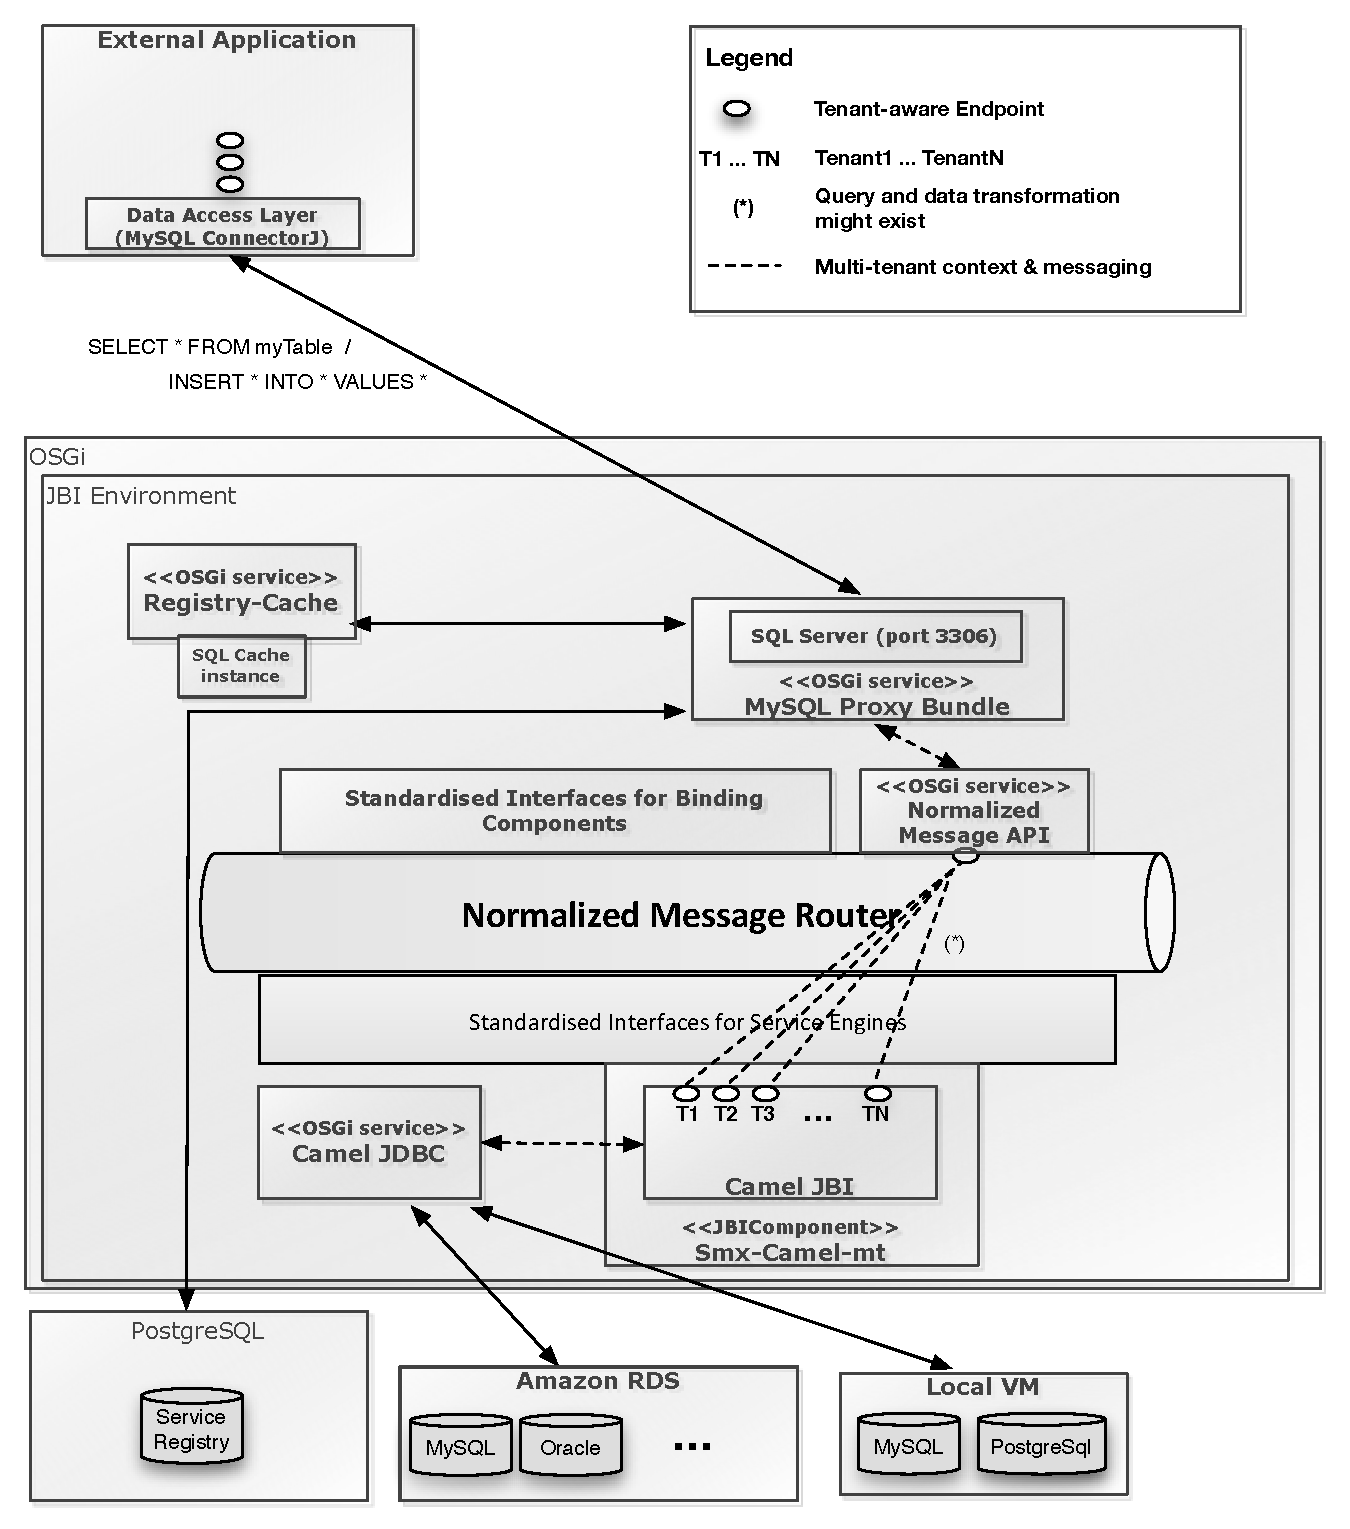
\includegraphics[clip, scale=0.6]{./gfx/sqlApproach/sqlApproachv2_doc.pdf}
	\caption[SQL Support Approach 1]{Architectural overview of the design approach one to support the MySQL communication protocol and routing to backend \ac{SQL} databases.}
	\label{fig:designsqlapp1}
\end{figure}

Apache Camel provides a set of components which integrate most of the communication technologies available in the market. Moreover, it provides an archetype for creating custom components we use in this diploma thesis. ServiceMix provides a Camel \ac{JBI} \ac{BC} which integrates the \ac{JBI} container with the camel router. Muhler extends this component in ServiceMix-mt and enriches it with multi-tenancy awareness. However, the supported multi-tenancy is at the level of tenants, and not at the level of tenant's users. We extend this component and provide user and tenant isolation between endpoints, by injecting the tenant and user UUID in the endpoint's URI (see Listing \ref{lst:endpointuri}). 

%%%%%%%%%%%%%%%%%%%%%%%%%%%%%
\lstinputlisting[float=htb,label={lst:endpointuri},caption={[Tenant-aware Endpoint Configuration]Extended Tenant-aware endpoint URI in extended Backus-Naur Form (EBNF) \cite{Muhler2012}.},style=ebnf]{./gfx/endpointconfiguration.txt}
%%%%%%%%%%%%%%%%%%%%%%%%%%%%%

With multi-tenancy at the tenant and user level, each user can deploy one \ac{JBI} tenant-aware endpoint in the ServiceMix-Camel-mt \ac{SE}. The routes deployed from each tenant-aware endpoint are performed under a different context, and an instance of the targeted component in the route is created. Therefore, with this approach we provide multi-tenancy at the messaging, endpoint, and routing and component context levels. 

Due to the lack of \ac{JDBC} support in ServiceMix for creating provider endpoints, we develop a custom camel component, and enrich it with \ac{JDBC} support for three database systems: MySQL, Oracle, and PostgreSQL. This component is extensible to more database systems when including its native driver, and is build as an \ac{OSGi} bundle and its packages are exported as an \ac{OSGi} service. Messages received from the \ac{NMR} are demarshaled to the backend database system communication protocol, and the response marshaled, correlated, and sent back to the MySQL Proxy Bundle. The demarshalers in this bundle provide the necessary support for transforming the \ac{NMF} response to a MySQL message.

As described in the previous section, ServiceMix-mt provides \ac{JBI} and \ac{OSGi} support and integration, but with some constraints. \ac{JBI} components cannot import packages from \ac{OSGi} bundles exporting its packages. The Servicemix-Camel-mt \ac{SE} provides integration with the camel router for a set of camel components. The camel manual specifies the need for adding statically the custom component packages in the \ac{JBI} \ac{SU} which contains the route definition. Therefore, this leads us to scalability problems in each of the \ac{SA} deployed by the tenants. The \ac{SA} size increases with the new supported database systems, and forces to redeploy all the \ac{SU}s containing the custom camel component when it is modified. This leads to management, storage capacity, and network capacity inconveniences. Hence, we provide a second, and final approach which is very similar to this one, but utilizing the ServiceMix-camel component deployed as \ac{OSGi} bundle. 

\FloatBarrier

\subsection{Approach 2}

In this second architectural design approach we address the scalability problems caused by the \ac{JBI} package dependencies in the \ac{SU}s described in the previous section. This approach is similar to the first one presented, and its main difference relies on the routing from the tenant-aware \ac{JBI} endpoints to the custom camel component \term{cdasmixjdbc} (see Figures \ref{fig:designsqlapp2} and \ref{fig:designsqlapp1}). The functionalities and operations in the MySQL proxy bundle do not differ with the previous approach.
 
\begin{figure}[htb]
	\centering
		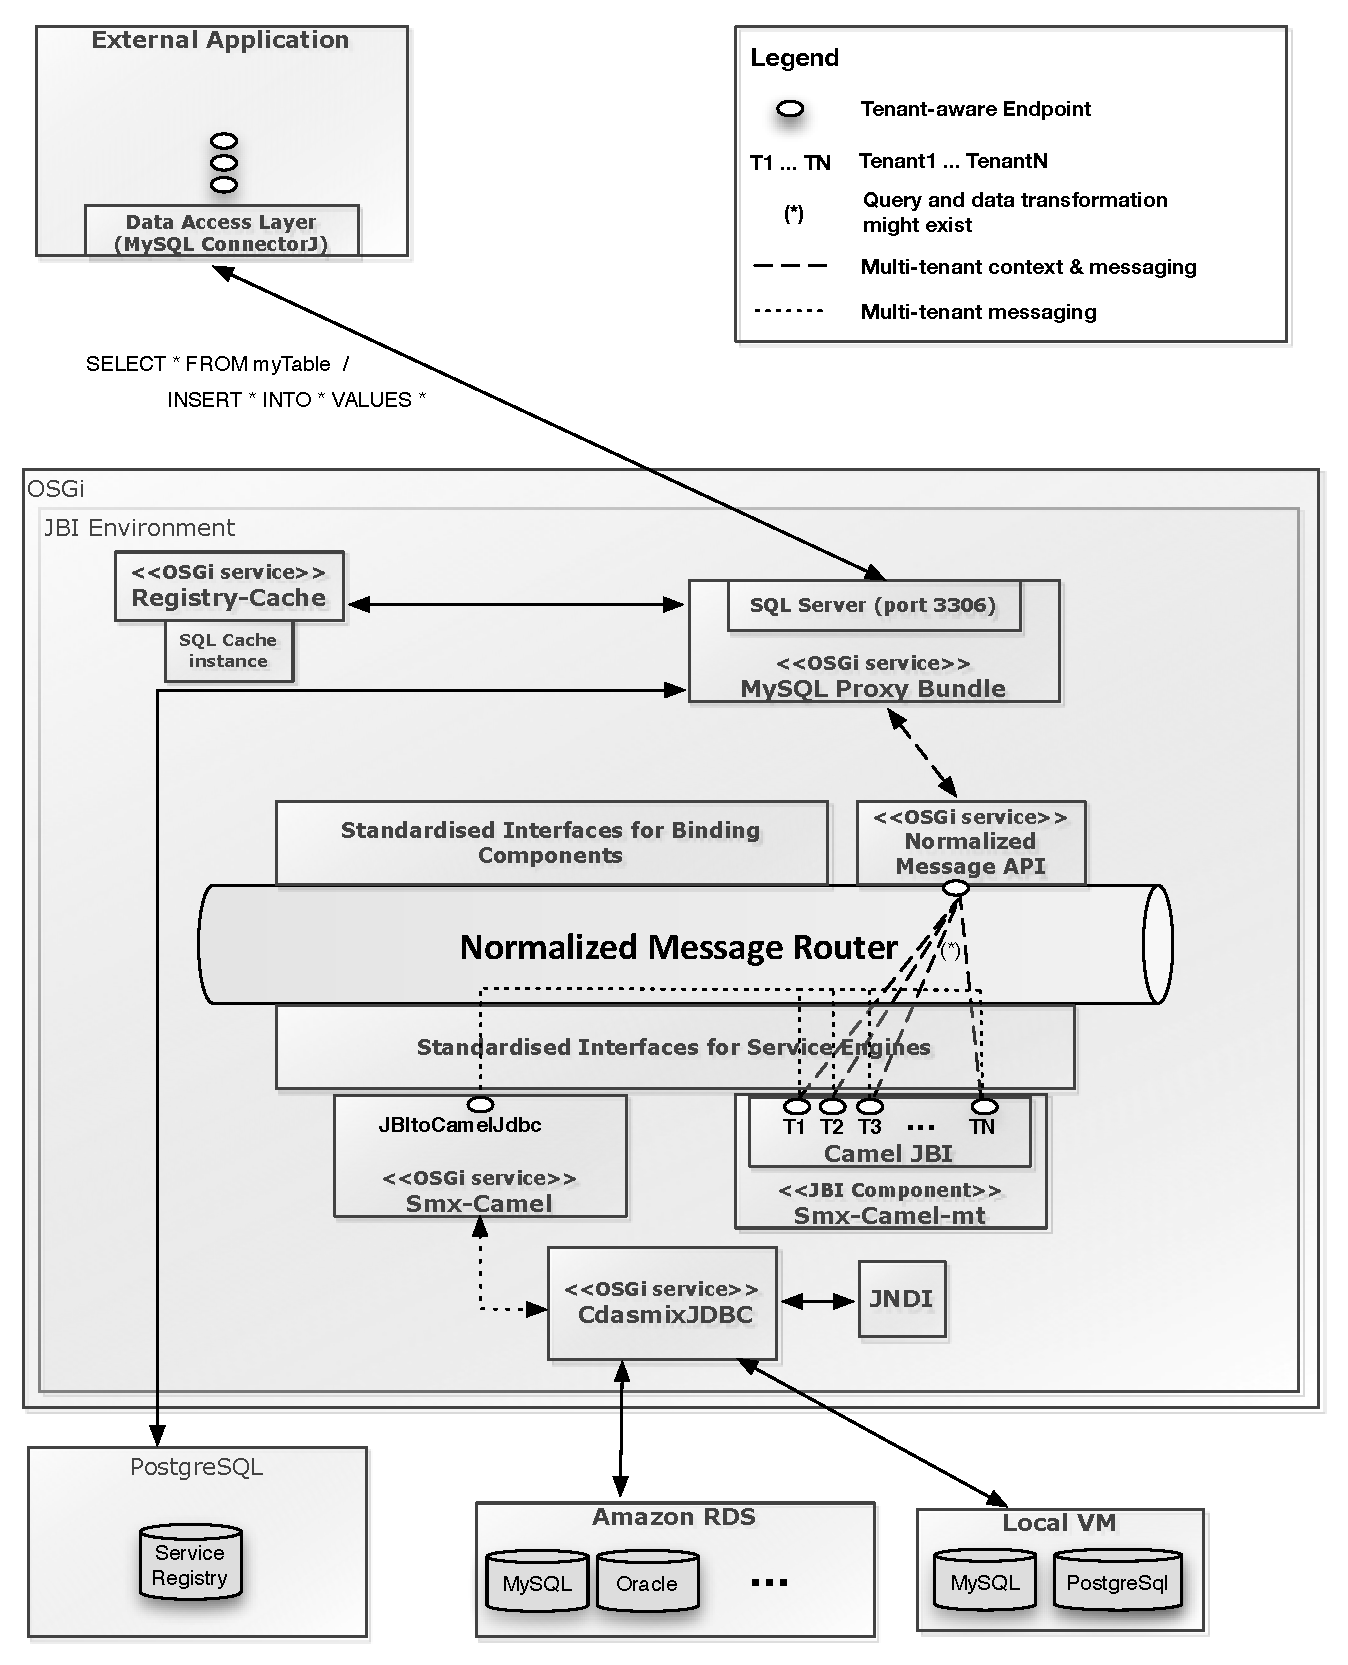
\includegraphics[clip, scale=0.6]{./gfx/sqlApproach/sqlApproachv3_doc.pdf}
	\caption[SQL Support Approach 2]{Architectural overview of the design approach two to support the MySQL communication protocol and routing to backend \ac{SQL} databases.}
	\label{fig:designsqlapp2}
\end{figure}

The message is routed from the MySQL proxy bundle to the tenant-aware \ac{JBI} endpoint deployed in ServiceMix-camel-mt. The multi-tenant message processor instance in ServiceMix-camel-mt routes the message to the \term{JBItoCamelJdbc} endpoint. 

As discussed before, the \ac{JBI} \ac{BC}s deployed in ServiceMix are \ac{OSGi} friendly. This means that the \ac{OSGi} contains a valid manifest file where the description of the bundle, import packages, and export packages are specified. \ac{SU}s deployed on this component are able to reference other \ac{OSGi} packages exposed as a service in the \ac{OSGi} service registry. We provide a single endpoint deployed in the ServiceMix-Camel component where the requests are sent to: the \term{JBItoCamelJdbc} endpoint. When the \term{JBItoCamelJdbc} endpoint is deployed on the ServiceMix-Camel \ac{OSGi} bundle, this searchs in the \ac{OSGi} container for the \term{CdasmixJDBC} component, and creates an instance of the component. Messages routed to the \term{JBItoCamelJdbc} endpoint are then forwarded to the \term{CdasmixJDBC} component, which selects the appropriate \ac{JDBC} native driver, creates a connection, demarshals the request, and forwards the request to the backend Cloud data store server. The connection is established after creating an instance of a \term{DataSource}, which is saved in the \ac{JNDI} registry for future connections, in order to avoid the creation of more than one \term{DataSource} instance per user per backend Cloud data store.

Responses retrieved from the backend Cloud data store are correlated with the initial request and routed back to the MySQL proxy bundle, which demarshals the retrieved data and sends it as a binary \ac{TCP} stream.

In this approach a new instance of the \term{cdasmixjdbc} is not created per tenant endpoint, but is shared between the tenants. Therefore, we cannot ensure an independent component context at the provider endpoint. However, messages contain the tenant information, and the \term{cdasmixjdbc} component interacts with the backend database system establishing separate \ac{JDBC} connections per request. Full multi-tenancy, at the levels of component creation, and endpoint level is not ensured, but it is ensured at the messaging, and context levels. Although full multi-tenancy is not supported, we avoid the deployment of \ac{SU}s which contain the \term{CdasmixJDBC} component in it, and whose size increase may lead to scalability problems in the system. Furthermore, we prevent the deployment of the same component n times, for the n multi-tenant aware endpoints, and prevent future management problems when modifying or upgrading the \term{CdasmixJDBC} component. 

\FloatBarrier


